\section{Durchführung}
Zur Aufnahme der Messreihen wird ein XY-Schreiber
verwendet. Zur Justierung für den Nullpunkt wird der
Knopf "Zero" benutzt ebenso werden die Achsenskalierungen
so eingestellt, dass sie ausgewertet werden können.
Um das Kontaktpotential bestimmen zu können, wird zunächst der
Versuch bei Umgebungstemperatur von ca. 25,4 Grad sowie die Beschleunigungsspannung $U_b$
auf +11 V eingestellt. Dabei wird der Strom $I_a$ in Abhhängigkeit der Bremsspannung $U_a$ aufgezeichnet.
Um eine Energieverteilung zu bestimmen wird die Temperatur mit Hilfe einer Heizung erhöht und die Aufzeichnung
erfolgt wie eben beschrieben ist.
\begin{figure}
  \centering
  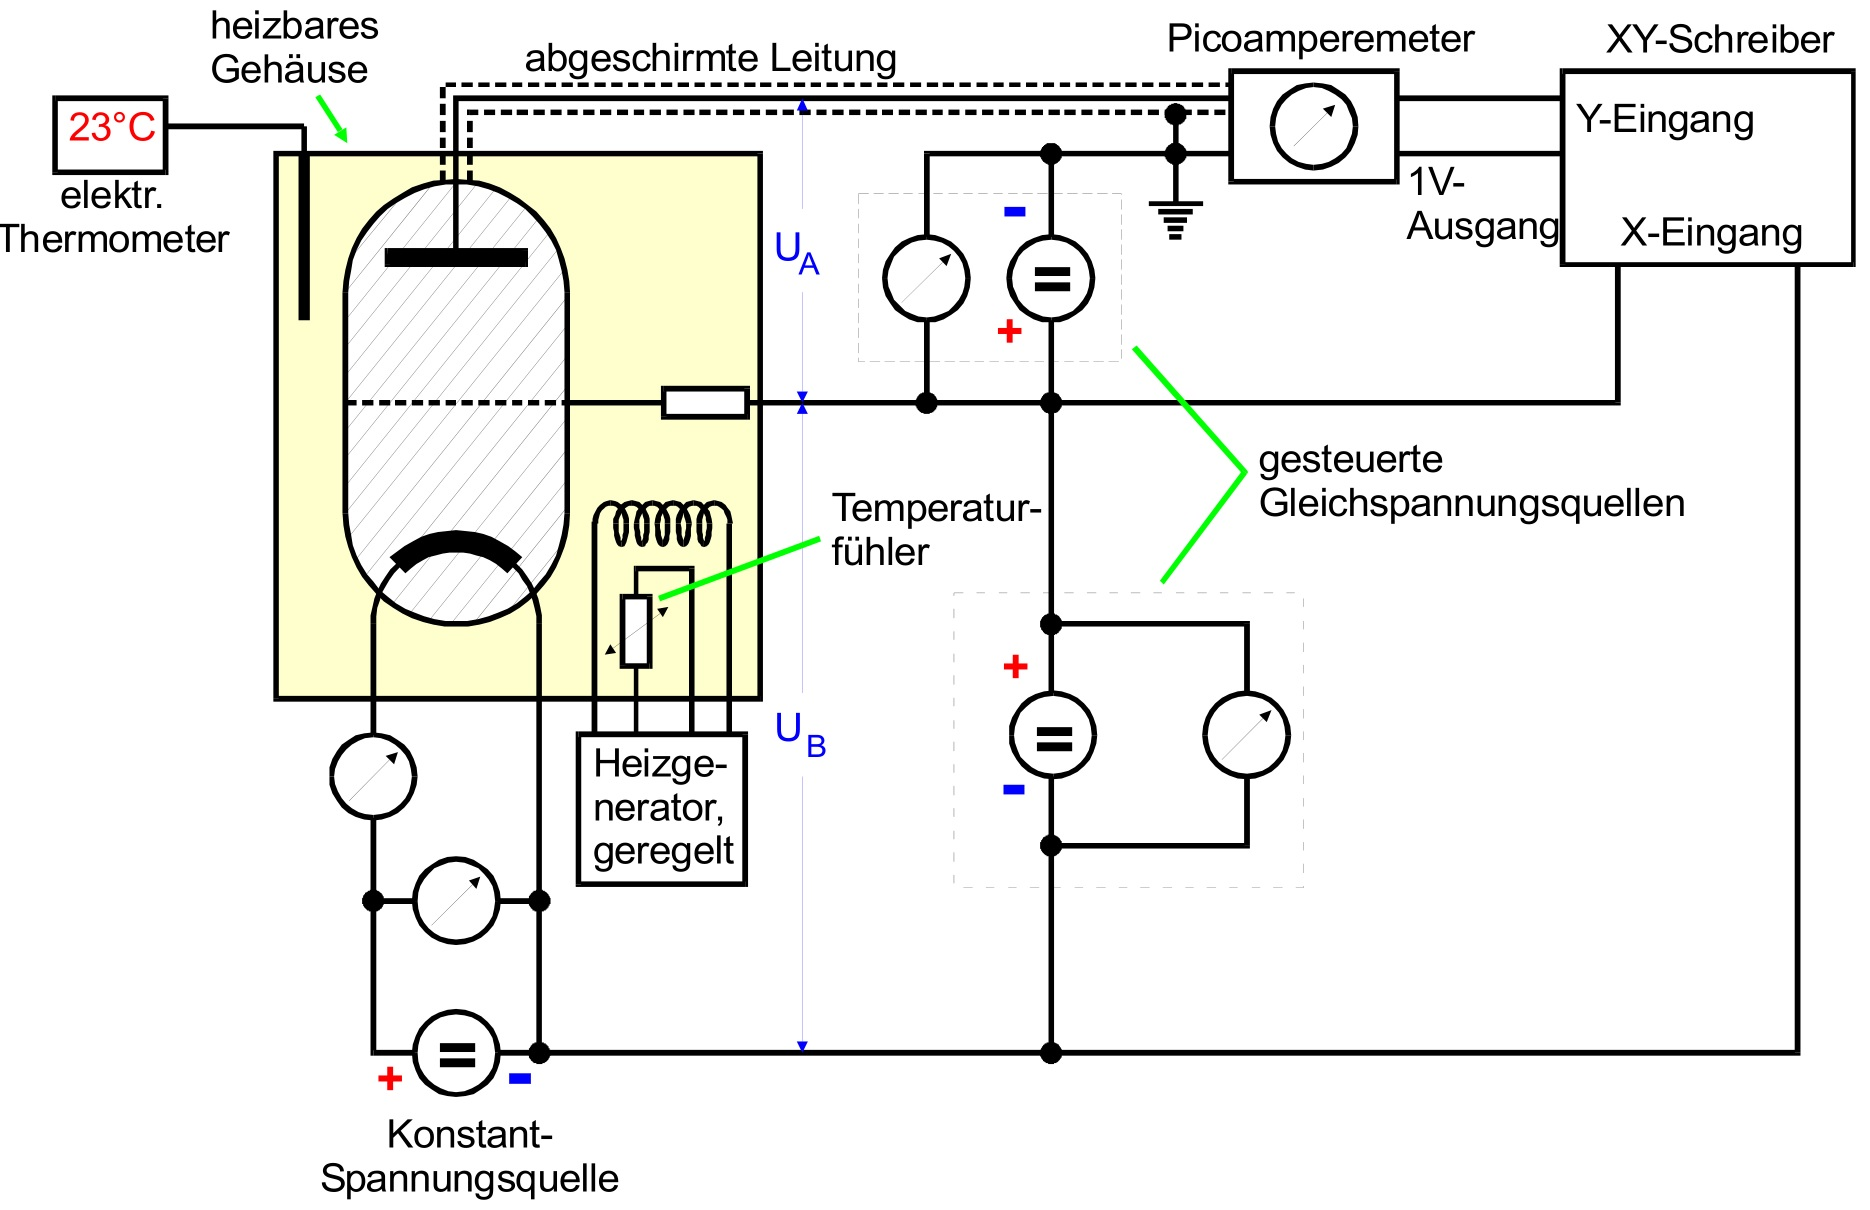
\includegraphics[width = 7 cm , height = 5.5 cm]{content/Anleitung.jpg}
  \caption{Aufbau zur Bestimmung der Frank-Hertz-Kurve \cite{1}.}
  \label{abb:3}
\end{figure}
In Abbildung (\ref{abb:3}) ist eine Dastellung zur Aufnahme der Kurve. Die Temerpatur im evakuiertem Gefäß muss so gegeben sein,
dass bei der Erhöhung der Beschleunigungsspannung $U_b \text{auf} + 60 V$ einen Stromwert von 1 -3 nA besitzt.
Anschließend wird der Strom $I_a$ in Abhhängigkeit der Beschleunigungsspannung $U_b$ mit dem XY-Schreiber aufgenommen.
Um die Ionisationsenergie des Hg-Atoms zu bestimmen, wird die Bremsspannung auf den Wert von -30 V eingestellt.
Dies führt dazu das die Elektronen bei der Auffängerelektrode nicht detektiert werden sondern nur die Atomionen registriert werden.
Die Temperatur muss dabei so eingestellt werden, dass die bei 100 - 110 Grad liegen soll.
Anschließend wird der Strom $I_a$ erneunt in Abhhängigkeit der Beschleunigungsspannung $U_b$ aufgezeichnet.
